\begin{chapter}{Evaluation}
	\label{chapter:Evaluation}

	This chapter will present an adaptation of the examples provided in \cite{mauborgne:rival05} as well as a short evaluation of the performance impact the trace partitioning has on the static analysis. As previously mentioned, array accesses are not yet precisely supported in \sample but required for the following examples. One way to work around this problem is to make pseudo array accesses. Listing \ref{listing:Array::access} depicts a normal array access in \scala.
	
	\lstinputlisting[float=h, caption=Normal Array Access, label=listing:Array::access]{Source/Array_access.scala}

	To illustrate what is meant by pseudo array access, Listing \ref{listing:Array::pseudoAccess} replicates the same behavior without having to call any access methods and is therefore analyzable using \sample. 

	\lstinputlisting[float=h, caption=Pseudo Array Access, label=listing:Array::pseudoAccess]{Source/Array_pseudoAccess.scala}

	The \code{return 0} statement in line \code{8} represents the exceptional control flow in case the index is out of bounds. This will result in an exit state and its execution will not interfere with the rest of the analysis. Note that, due to the verbose nature of this access, it is shortened in the following examples wherever logically possible.

		Furthermore, since the only numerical type supported by \sample at the moment is \code{Int}, the adapted examples using linear interpolation will not be using floating point numbers as in their original presentation but are limited to integers. However, the principles behind the examples remain the same. Once \sample supports \code{Float}, all that needs to be changed are the type declarations in the guest domain.

	Although the guest domain used in this chapter is once more the interval domain, this need not be the case. It has, however, the advantage that it is a very intuitive domain and can easily be visualized and understood.

	% Partitioning a Conditional

	\begin{section}{Partitioning a Conditional}
		The first example here is also the introductory example that was already used to illustrate the extended transition system. The method of interest is shown in Listing \ref{listing:Examples::ifExample}
	
		\lstinputlisting[float=h, caption=The \code{ifExample} Method, label=listing:Examples::ifExample]{Source/Examples_ifExample.scala}

		The property of interest is whether or not there could be an unsafe division in this method. That is, is there a division where the divisor could possibly be zero? Intuitively, there is no such division. Proving so, especially using common numerical abstract domains, turns out to be surprisingly complicated.

		The division occurs in line \code{8} and the divisor is the \code{sign} variable. At the beginning of the analysis, no assumptions about the value of the variable can be made, thus \code{sign} is represented by $\top$ or, when using an interval domain, the equivalent \code{[-inf,inf]} interval. After simulating line \code{2}, the value of \code{sign} is clearly zero, hence it will be represented by \code{[0,0]}. Continuing, the flow of control is split into the \code{true} and \code{false} branch of the conditional. At the end of the branches, the value lies in \code{[-1,-1]} and \code{[1,1]} respectively. Joining the two branches just before the division leads to the interval \code{[-1,-1] $\sqcup$ [1,1] = [-1,1]}. This interval obviously contains the zero and the analysis generates a warning when looking at the statement in line \code{8}.

		A whole class of commonly used domains, called convex domains, follows along the same line of reasoning and thus fails to prove this seemingly trivial property. More complex domains can provide a solution but are usually prohibitively expensive.

		Inserting a \code{PartitionIf} directive for the condition in line \code{3} (more precisely at position \code{(3,13)}) will distinguish traces following either of the conditional branches. Figure \ref{figure:PartitionIfExample} illustrates the concrete key states of the partitioned analysis.

		\begin{figure}
			\centering
			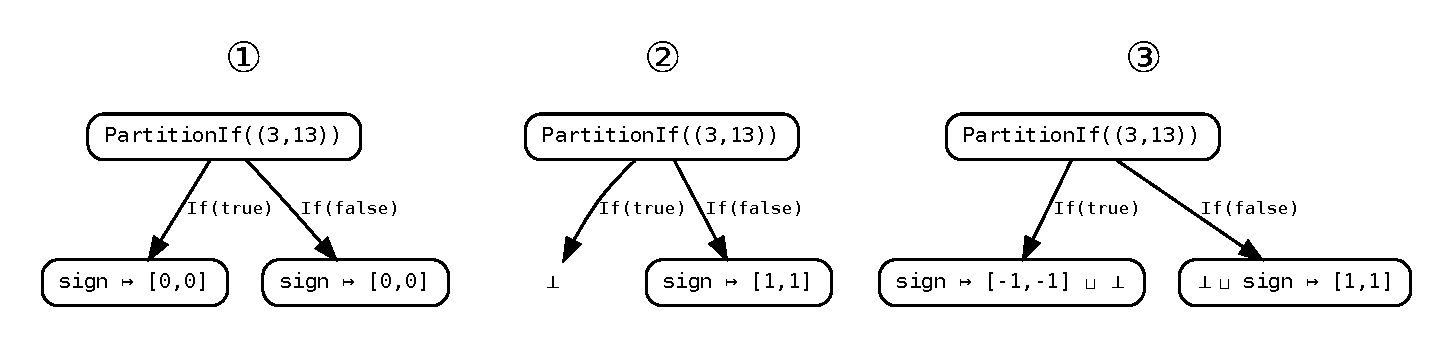
\includegraphics[width=\textwidth]{Graphs/PartitionIfExample.pdf}
			\caption{Key States of the Analysis}
			\label{figure:PartitionIfExample}
		\end{figure}

		Up to the conditional statement, the analysis starting with a partitioned state in form of a leaf containing the interval state is completely equivalent to the analysis just described. Once the conditional is encountered, the directive will take effect and split the leaf into a node with two children. The graph \one illustrates the state after analyzing line \code{3}. The partitioned state is then passed through the branches by applying the \code{testTrue} or \code{testFalse} method and subsequently the semantic function of the respective branch's single statement. The state at the end of the \code{false} branch is depicted in \two. The result from the \code{true} branch looks similar, but with a leaf for the \code{If(true)} token containing the interval \code{[-1,-1]}. Before inspecting line \code{8}, the two branches are joined. \three shows how the guest states are combined leaf-wise using the least upper bound. The analysis then successfully proves that the division in line \code{8} is safe.
	\end{section}

	% Partitioning Over a Variable

	\begin{section}{Partitioning over a Variable}
		The second example here is concerned with the evaluation of the following piecewise linear interpolation function.
		\begin{align}
			f(x) = 
				\begin{cases}
					-1 - x & \text{if } x < -1 \\
					-1 + x & \text{if } x > 1 \\
					0 & \text{otherwise}
				\end{cases}
		\end{align}

		\begin{figure}
			\centering
			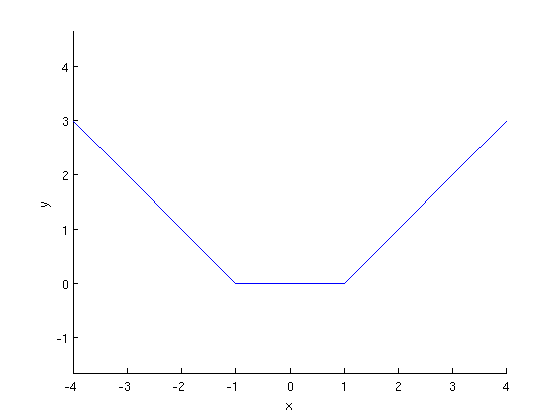
\includegraphics[scale=0.7]{Plots/valueExample.png}
			\caption{The Piece-Wise Linear Function}
			\label{figure:valueExample}
		\end{figure}

		A plot of the function is given in Figure \ref{figure:valueExample}. An implementation of this function evaluates the function as $f(x) = c_i + m_i x$, with coefficients determined by the interval $x$ lies in. Starting with the somewhat cumbersome array workaround presented earlier and drastically simplifying it, this method leads to the code displayed in Listing \ref{listing:Examples::valueExample}.

		\lstinputlisting[float=h, caption=The \code{valueExample} Method, label=listing:Examples::valueExample]{Source/Examples_valueExample.scala}

		The point of interest in this example is the value of \code{y} at the end of the method. To have a point of comparison it is once more helpful to quickly step through the analysis using the normal, non-partitioned interval domain. At the beginning, nothing is known. All values are assumed to have the value of $\top$, represented by \code{[-inf,inf]}. Executing the initial assignments, that is lines \code{2} to \code{3}, leads to a state where the value of \code{x} is still undefined and that of \code{y}, \code{c} and \code{m} is \code{[0,0]}. Since nothing is known about x, the four consecutive conditionals are not determined and \code{c} ends up in the interval \code{[-1,0]} while \code{m} is assumed to be somewhere in \code{[-1,1]}. This information is utterly useless once line \code{12} is reached because \code{x} could have any value and the slope could be anything from \code{-1} to \code{1}. The analysis therefore concludes that the resulting \code{y} must lie in the interval given by \code{[-inf,inf]}. Looking at the plot, this result is disappointing and unnecessarily inaccurate.

		\begin{figure}[t]
			\centering
			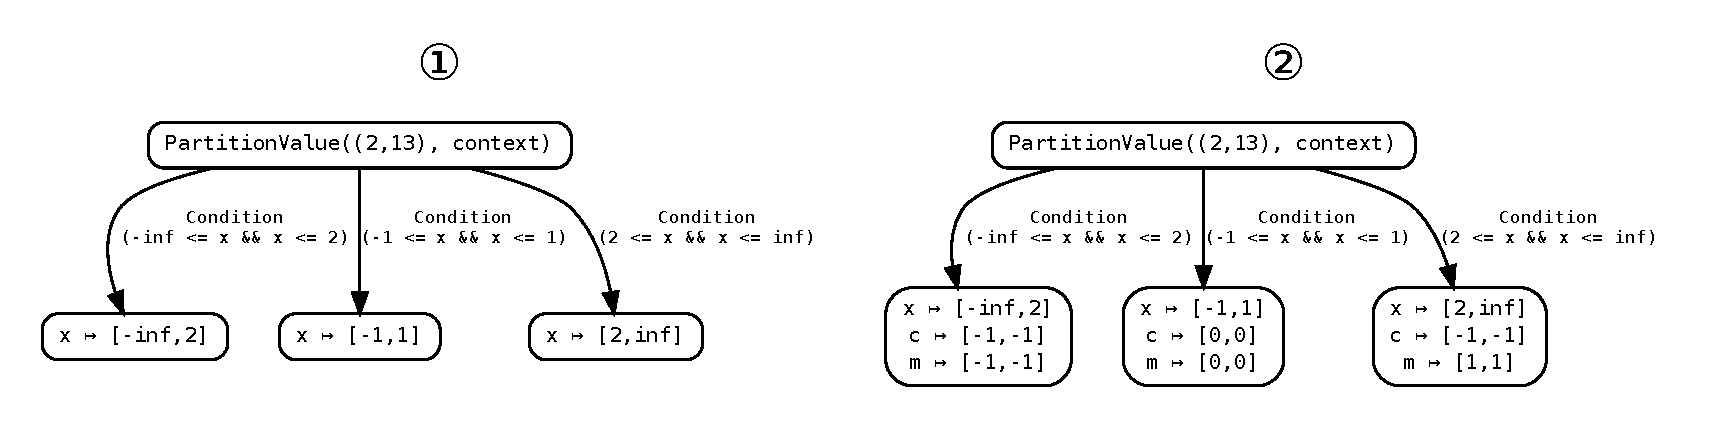
\includegraphics[width=\textwidth]{Graphs/PartitionValueExample1.pdf}
			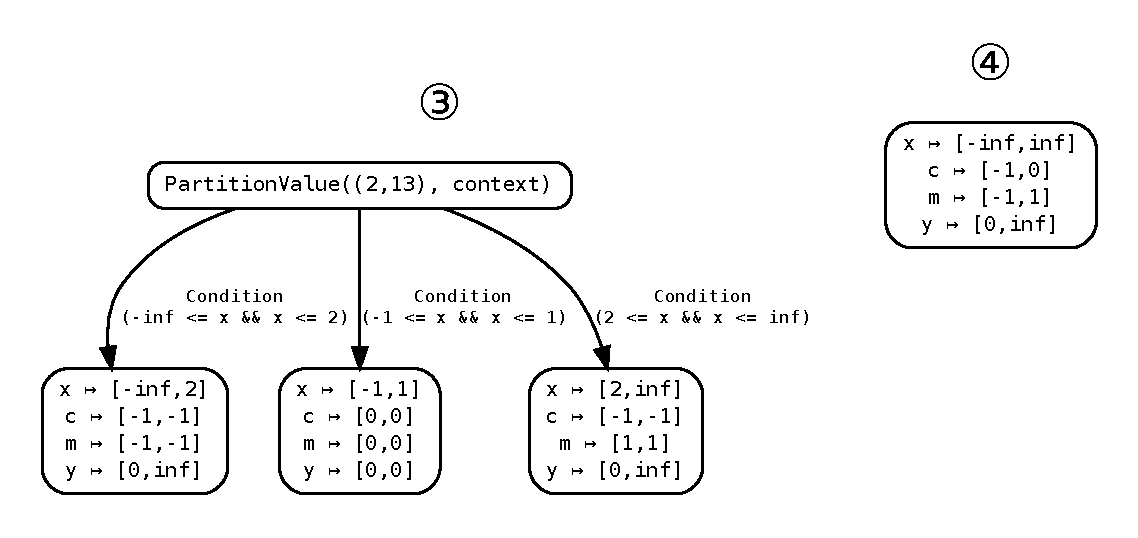
\includegraphics[scale=0.5]{Graphs/PartitionValueExample2.pdf}
			\caption{Analysis with a \code{PartitionValue} Directive}
			\label{figure:PartitionValueExample}
		\end{figure}

		Inserting a \code{PartitionValue} directive at the beginning of the method and a \code{Merge} directive before returning the result leads to the key states depicted in Figure \ref{figure:PartitionValueExample}. The directive here is applied before the first assignment and distinguishes the three intervals \code{[-inf,2]}, \code{[-1,1]} and \code{[2,inf]} for the variable \code{x}. Note that since the method works with integers, these intervals cover the whole range of possible values. The initial partitioned state is depicted in \one. The leaves simply represent the assumptions made by the partitioning directive. Continuing with the partitioned state, the analysis gains in precision when accessing the coefficient arrays as is shown in \two, the state right before the polynomial evaluation. The state afterwards, depicted in \three, infers that, for \code{x} smaller than \code{-1} or greater than 1, \code{y} must be positive, and zero otherwise. Merging the directive results in the leaf depicted in \four. While merging leads to a loss of information, it is still possible to infer that \code{y} is always greater or equal to zero, which is exactly the purpose of this analysis.

		Note that although the intervals for the directive chosen for this illustration coincide with the definition intervals of the linear interpolation function, this is not necessary to gain precision in the analysis. Even a split of \code{x} into a positive and negative interval would lead to a better result, though it would no longer be possible to prove the lower bound of zero (but that of \code{-1}).
	\end{section}

	% Partitioning a Loop

	\begin{section}{Partitioning a Loop}
		The third example is very similar to the previous one in that it is also concerned with the evaluation of a piecewise linear function. The function in question is defined as
		\begin{align}
			f(x) = 
			\begin{cases}
				x & \text{if } 0 \leq x < 2 \\
				4 - x & \text{if } 2 \leq x < 4 \\
				0 & \text{otherwise}
			\end{cases}
		\end{align} 
		and plotted in Figure \ref{figure:whileExample}.

		\begin{figure}
			\centering
			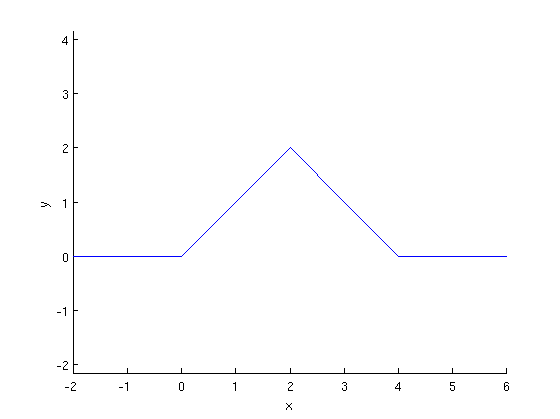
\includegraphics[scale=0.7]{Plots/whileExample.png}
			\caption{The Piece-Wise Linear Function}
			\label{figure:whileExample}
		\end{figure}

		Once more, the linear functions are represented by coefficients $c_i$ and $m_i$ for four intervals stored in an array. The main difference to the example before is how the index for accessing the coefficients is computed. The idea is to store the upper bound of the interval in a special array \code{iv} and increase the index \code{i} until \code{iv(i+1)} is no longer bigger than \code{x}. This array for the function above would then be \code{Array(0, 2, 4, 6)}. The regularity of this array was chosen in order to alleviate this presentation of one more pseudo array access than necessary. The final code evaluating the function is shown in Listing \ref{listing:Examples::whileExample}.

		\lstinputlisting[float=h, caption=The \code{whileExample} Method, label=listing:Examples::whileExample]{Source/Examples_whileExample.scala}

		Without a partitioned state, the analysis has very limited power. As always, starting with $\top$ for all variables and analyzing the initializing statements \code{x} has the value \code{[-inf,inf]} and all other \code{[0,0]}. The while loop only affects the \code{i} variable and knowing that the loop is executed at most three times, the analysis will conclude that \code{i} must be in the interval \code{[0,3]}. Unfortunately, this leads to all possible combinations for the pseudo array accesses and finally the conclusion that \code{y} can have any value whatsoever.

		Partitioning over the value of \code{x} does not improve the analysis. Consider the leaf for the token \code{Condition(2 <= x \&\& x <= 3)}. The state will be analyzed every time the fixed point iteration iterates through the loop. The first time \code{i} is determined to be in the interval \code{[1,1]}. The second iteration will then join that result with the newly determined interval \code{[2,2]} and hence result in \code{[1,2]}. The last iteration will add \code{3} to the interval and combined with the state skipping the loop altogether the resulting state will map \code{i} to \code{[0,3]}, which is exactly what happened without a partitioning.

		\begin{figure}
			\centering
			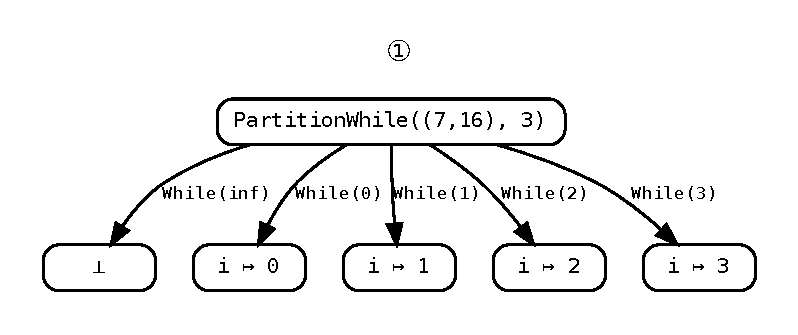
\includegraphics[]{Graphs/PartitionWhileExample1}
			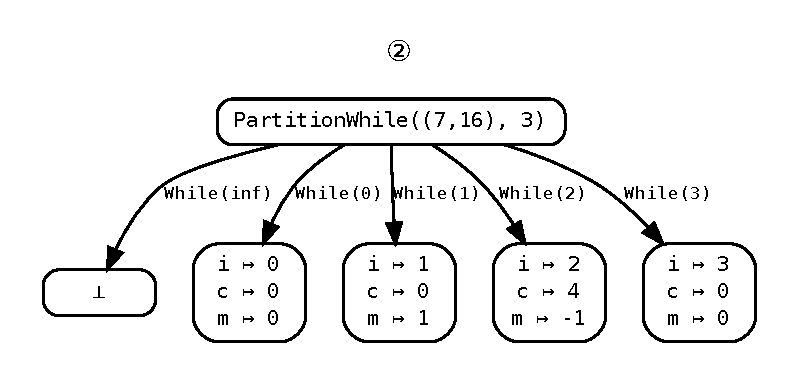
\includegraphics[]{Graphs/PartitionWhileExample2}
			\caption{Analysis with a \code{PartitionWhile} Directive}
			\label{figure:PartitionWhileExample}
		\end{figure}

		The sensible thing to do is therefore to partition over the different executions of the loop statement. Knowing that the array index can have at most four values, distinguishing the traces leading to those four values is a good choice. The state \one in Figure \ref{figure:PartitionWhileExample} shows a simplified version of the state after the loop has been analyzed. The fact that the loop is never executed more than three times is reflected in the state for the token \code{While(inf)} where it leads to a contradiction. Before evaluating the polynomial, the pseudo array accesses determining the values of \code{c} and \code{m} are executed and lead to state \two. So far, the value of \code{x} has been neglected in this analysis. It is determined by what the underlying domain can conclude from assuming the loop condition. For this example it is \code{i < (x+2)/2}, which is merely enough to prove that in the end after merging the directive \code{y} will always be greater than \code{-4}. Even with this imprecision caused by the array workaround, the result is a serious improvement over the non-partitioned analysis.

	\end{section}

	% Performance 

	\begin{section}{Performance}
		\label{section:Performance}

		It is inherently difficult to make any qualitative statements about the performance of the trace partitioning implementation. The convergence of the fixed point iteration is highly dependent on the inserted directives and the chosen widening limits set for the fixed point iteration as well as for the trace partitioning mechanism. 

		Ignoring the widening limits, having no directives and performing the analysis with an initial partitioned state in form of a leaf simply adds the constant cost of redirecting the calls to the state interface to the enclosed guest state. On the other hand, having a \code{PartitionIf} directive inside a loop without a corresponding \code{Merge} directive leads to an exponential blow-up. 

		Further complications in estimating the running time stem from the fact that a significant gain in precision can also lead to a significantly faster convergence as was observed by Mauborgne and Rival. Again, this heavily depends on the chosen directives, a problem that is further addressed in Section \ref{section:OpenQuestions}.

		Using a large body of methods to analyze and some heuristics to automatically generate directives would permit a more useful analysis. Unfortunately, two requirements for this to be feasible are not yet fulfilled. For one, \sample is not yet ready to deal with real world code making analysis of a large body of code difficult (cf. Section \ref{section:Limitations}). Moreover, the trace partitioning implementation still depends on manually generated directives and is therefore unable to act unsupervised, limiting its applicability to bigger code.

		Mauborgne and Rival evaluated their implementation on large projects containing up to 400'000 lines of code using heuristically inserted directives. Their results show a great increase in precision, and a significant decrease of iterations used in some but not all of the analyses.
	\end{section}
\end{chapter}
